\definecolor{Gray}{gray}{0.9}

\chapter{Analisi del dominio}
Questo capitolo verte su tutta l'analisi impiegata sulla conoscenza del dominio dell'applicativo, sull'identificazione dei requisiti, dei casi d'uso nonché sull'analisi dei principi della filosofia Domain Driven Design. \newline \newline Questa fase è stata di grande importanza poiché ci ha permesso, da una parte di avere un ottima conoscenza del dominio applicativo e dall'altra di discutere sui principali aspetti di sviluppo agevolando notevolmente la successiva fase di implementazione.

\section{Il dominio}
In questa sezione verrà descritto il dominio dell'applicativo: verrà presentato l'obiettivo da raggiungere, lo stato dell'arte e l'\textit{ubiquitous language} individuato.
 
\subsection{Obiettivo}

L'obiettivo del progetto è la creazione di un sistema che consenta a tutto il team della sala operatoria (medici, infermieri e anestesisti) di accedere in maniera agevole a tutte le informazioni del paziente durante un intervento chirurgico. In particolare quello che si richiede è di poter virtualizzare attraverso un ologramma il monitor a parametri vitali del paziente. In questo modo, durante un intervento, ogni membro del team può visualizzare ed interagire con l'ologramma controllando i relativi valori dei parametri del monitor indipendentemente dalla locazione del dispositivo fisico. \newline \newline Questo approccio porta a semplificare tutta una serie di operazioni che possono essere svolte sul paziente durante l'operazione. Si pensi se durante un intervento è necessario eseguire una TAC d'urgenza: significherebbe trasportare il paziente, tutti i sensori a cui è collegato e il relativo monitor in una stanza adiacente a quella chirurgica con il rischio di perdere del tempo prezioso per problemi che possono incorrere durante il trasferimento. Se si adottasse la soluzione proposta, sarebbe necessario spostare solamente il paziente e non i dispositivi fisici poiché ogni membro del team continua a visualizzare l'ologramma, riducendo così il tempo impiegato nel trasferimento del paziente.
Un altro vantaggio è dato dalla connessione in remoto allo stato del monitor del paziente da parte di altri medici che possono essere coinvolti nell'operazione.

\subsection{Stato dell'arte}
Molte grandi città del mondo stanno già impiegando questa tecnologia in ambito sanitario. Ad esempio nell'ospedale di Singapore, i chirurgi utilizzano questo approccio per visualizzare ologrammi di referti dei pazienti (come una risonanza magnetica) durante un intervento chirurgico (maggiori informazioni a questo \href{https://govinsider.asia/citizen-centric/how-a-singapore-hospital-uses-holograms-to-assist-surgery-nuhs-ngiam-kee-yuan/} {\textit{link}}). Si tratta di un caso simile al nostro ma con una principale differenza: nel nostro caso l'ologramma viene aggiornato in \textit{real-time} con i dati del paziente.\newline

\begin{wrapfigure}{l}{0.4\textwidth}
    \centering
    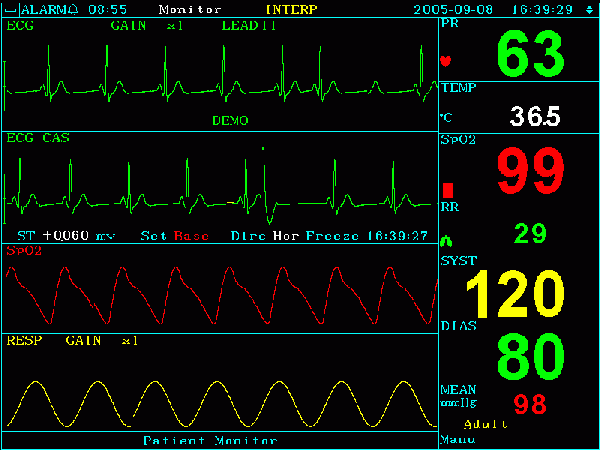
\includegraphics[width=0.4\textwidth]{monitor.png}
    \caption{Esempio di monitor a parametri vitali.}
    \label{pic:monitor_example}
\end{wrapfigure}

Durante l'intervento, al paziente vengono collegati diversi sensori per monitorare i parametri vitali. \newline I valori dei parametri vengono mostrati nel monitor ognuno con uno specifico colore. In particolare per ogni parametro viene mostrato il valore puntuale, l'unità di misura e per alcuni di loro anche un grafico. \newline Nella figura \ref{pic:monitor_example} è presente un esempio di monitor a parametri vitali ed è quello a cui noi ci siamo basati per la parte di simulazione. I parametri vitali monitorati sono: la temperatura, la pressione sanguigna, la frequenza respiratoria e cardiaca e la saturazione. Per ognuno di questi si è deciso anche di aggiungere un allarme che si attiva qualora il relativo valore supera una certa soglia sia inferiormente che superiormente.

\subsection{Ubiquitous Language}
L'\textit{ubiquitous language} contiene un insieme di termini usati nella definizione del dominio al fine di eliminare incertezze, imprecisioni e fraintendimenti che possono derivare da ogni membro del team di progetto, esperti del dominio e altri partecipanti. E' importante non solo specificare il significato di un termine ma anche il suo contesto di utilizzo. Tale linguaggio è sempre in continuo aggiornamento anche durante tutta la fase di sviluppo e non definito solamente all'inizio. \newline \newline La tabella \ref{tab:mixed-reality-ubiquitous-language-table} illustra l'\textit{ubiquitous language} per il nostro applicativo.

\bgroup
\def\arraystretch{1.5}
\begin{table}[H]
    \begin{tabular}{ |m{3cm}|m{3cm}|m{5cm}| } 
        \hline
        \textbf{Termine} & \textbf{Equivalenza} & \textbf{Descrizione}
        \\\hline
        Monitor a parametri vitali & Vital Signs Monitor & Monitor utilizzato per visualizzare i parametri vitali di un paziente durante un intervento chirurgico.
        \\\hline
        Dispositivi fisici &  Phisical Assets & Si intende il monitor a parametri vitali fisico e i relativi sensori.
        \\\hline
        Temperatura & Temperature & Parametro vitale riferito alla temperatura corporea del paziente che è possibile visualizzare nel monitor.
        \\\hline
        Saturazione & Saturation & Parametro vitale riferito alla saturazione del paziente che è possibile visualizzare nel monitor.
        \\\hline
        Pressione sanguigna & Blood Pressure & Parametro vitale riferito alla pressione sanguigna del paziente che è possibile visualizzare nel monitor.
        \\\hline
        Frequenza cardiaca & Heart Frequency & Parametro vitale riferito alla frequenza cardiaca  del paziente che è possibile visualizzare nel monitor.
        \\\hline
        Frequenza respiratoria & Breath Frequency  & Parametro vitale riferito alla frequenza respiratoria del paziente che è possibile visualizzare nel monitor.
        \\\hline
        Allarme &  Alert & Stato in cui si trova un parametro vitale quando il suo valore è troppo alto o troppo basso rispetto ad uno specifico range di valori impostato.
        \\\hline
        Unità di misura & Unit of measurement & Unità di misura utilizzata per rappresentare il valore di uno specifico parametro vitale.
        \\\hline
    \end{tabular}
\end{table}
\egroup

\bgroup
\def\arraystretch{1.5}
\begin{table}[H]
    \begin{tabular}{ |m{2.5cm}|m{2.5cm}|m{7cm}| } 
        \hline
        \textbf{Termine} & \textbf{Equivalenza} & \textbf{Descrizione}
        \\\hline
        Paziente & Patient & Persona che usufruisce del sistema realizzato.
        \\\hline
        Scheda Clinica & Medical Record & Documento che raccoglie le informazioni di tipo medico-anagrafico del paziente. 
        \\\hline
        Team & Team & L'insieme delle persone che utilizzeranno il sistema realizzato ovvero tutti i soggetti attivi nella sala operatoria durante un intervento chirurgico.
        \\\hline
        Ologramma & Hologram  & Rappresentazione tridimensionale dei dati nello spazio che consente l'interazione con essi.
        \\\hline
    \end{tabular}
    \caption{\label{tab:mixed-reality-ubiquitous-language-table}Ubiquitous language utilizzato nell'analisi del dominio.}
\end{table}
\egroup


\section{Requisiti}
Una delle fasi fondamentali dell’intero processo di analisi, è ricaduta nella definizione dei requisiti che il progetto dovrà soddisfare. Questi verranno raffinati in corso d’opera andando a creare una comprensione del dominio sempre più approfondita. Verranno descritti i requisiti di business, utente, quelli legati al sistema, funzionali e non funzionali.

\subsection{Business}
I requisiti di business sono così descritti:

\begin{itemize}
    \item Il prodotto dovrà fornire un monitoraggio a distanza. Questo consentirà al personale incaricato di poter controllare i parametri vitali del paziente in remoto;
    
    \item Il prodotto dovrà consentire di agevolare l'insieme delle operazioni svolte in sala operatoria che richiedono lo spostamento di dispositivi fisici;
    
    \item I dati mostrati nell'ologramma devono essere aggiornati in tempo reale, minimizzando il tempo di latenza.
\end{itemize}

\subsection{Utente}
I requisiti utente sono così descritti:

\begin{itemize}
    \item Il prodotto deve permettere di creare la scheda clinica del paziente quando questo viene ricoverato in ospedale;

    \item L'ologramma deve avere un interfaccia intuitiva simile il più possibile a quella di un monitor a parametri vitali fisico, con possibilità di un menù per poter fare un focus su uno specifico parametro vitale;
    
    \item L'ologramma deve avere un sistema di allerta se i valori dei parametri vitali sono al di sopra o al di sotto di uno specifico range;
    
    \item Il prodotto deve poter fornire la possibilità di personalizzare i parametri vitali. In particolare il personale incaricato potrà personalizzare il range di ogni parametro vitale e l'unità di misura con cui quel dato è rappresentato;
    
    \item L'ologramma dovrà mostrare la scheda clinica del paziente.
\end{itemize}

\subsection{Legati al Sistema}
I requisiti di sistema sono così descritti:
\begin{itemize}

    \item Il paziente deve poter essere identificato univocamente tramite il suo codice fiscale;
    
    \item L'accesso dello stato del paziente in sala operatoria tramite l'ologramma deve essere fatto per mezzo di un QR code.
\end{itemize}

\subsection{Funzionali}
Si elencano i requisiti funzionali per ognuno dei seguenti contesti:

\begin{itemize}
    \item Accesso del paziente in ospedale;
    \item Intervento chirurgico.
\end{itemize}

L'immagine \ref{pic:use-cases} mostra i caso d'uso del sistema relativi ai contesti citati.

\begin{figure}[ht]
    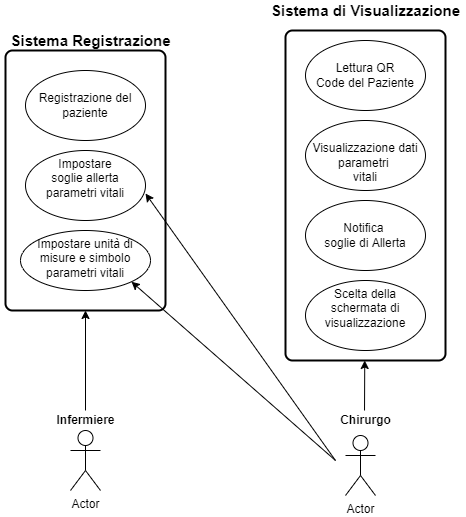
\includegraphics[width=11cm]{Images/useCase.png}
    \centering
    \caption{\label{pic:use-cases}Casi d'uso del sistema.}
\end{figure}

\subsubsection{Accesso del paziente in ospedale}
Quando il paziente deve essere ricoverato in ospedale è necessario registrarlo nel sistema informatico dell'ospedale. L'operatore incaricato dovrà quindi creare la sua scheda clinica compilando i dati richiesti. Successivamente, il chirurgo se lo ritiene necessario può configurare le soglie di allerta per i parametri vitali e infine si dovrà generare il relativo QR code che sarà utilizzato per il riconoscimento del paziente in sala operatoria.

\subsubsection{Intervento chirurgico}
Se è necessario eseguire un operazione chirurgica al paziente, il chirurgo può utilizzare oltre al monitor a parametri vitali fisico anche quello virtuale grazie alla visualizzazione di un ologramma. Per fare ciò sarà necessario scannerizzare il QR code del paziente (generato in fase di ricovero) sia nel monitor fisico sia nell'ologramma al fine di creare la connessione tra i due sistemi per la ricezione dei dati. In questo modo il chirurgo potrà visualizzare nell'ologramma i dati relativi ai parametri vitali del paziente, eventuali allarmi, i grafici, i valori puntuali e scegliere di monitorare un preciso parametro anziché avere una schermata generale di tutti. Inoltre sarà possibile visualizzare la scheda clinica del paziente compilata in fase di ricovero.

\subsection{Non funzionali}
I requisiti non funzionali sono così descritti.

\subsubsection{Usabilità}
Il sistema deve fornire agli utenti finali un’interfaccia chiara, semplice, ben organizzata in modo da poter utilizzare al meglio tutte le sue funzionalità messe a disposizione e visualizzate.

\subsubsection{Legati al Sistema}
\begin{itemize}
    \item \textbf{Reattività}. L'utente non deve percepire ritardi tra la visualizzazione dei dati nel monitor a parametri vitali fisico e la visualizzazione degli stessi nell'ologramma;
    
    \item \textbf{Fault tolerance}. Deve essere implementato un adeguato sistema di gestione degli errori affinché le interruzioni involontarie non compromettono la salute del paziente durante un intervento chirurgico;
    
    \item \textbf{Sicurezza}. Utilizzando \textit{Azure Digital Twins} i dati salvati nel cloud e quelli in transito tra due o più componenti di Azure sono crittografati;
    
    \item \textbf{Scalabilità}. L’applicativo deve necessariamente consentire di aumentare o diminuire il numero di pazienti gestiti senza influire negativamente sulla prestazione del sistema. 
\end{itemize}

\subsection{Implementativi}
Il software dovrà essere realizzato utilizzando la filosofia \textit{Domain Driven Design}. Dovranno inoltre essere utilizzate metodologie di DevOps al fine di automatizzare e integrare quanti più processi possibili. Si utilizzerà il servizio Azure Digital Twins (PaaS - Platform As A Service) per la gestione dei digital twins e l'interfacciamento con i diversi clients. Per la parte di mixed reality si utilizzerà la piattaforma Unity e i visori Microsoft Hololens 2.

\section{Aspetti di Domain Driven Design}

Partendo dall'analisi dei requisiti evidenziati al paragrafo precedente e dall'approfondimento dei processi che avvengono nel contesto ospedaliero, abbiamo cercato di semplificare il dominio in cui si deve implementare la nostra soluzione dividendolo in più sotto-domini, alcuni di questi di interesse per la nostra implementazione, altri non correlati.

\begin{figure}[H]
    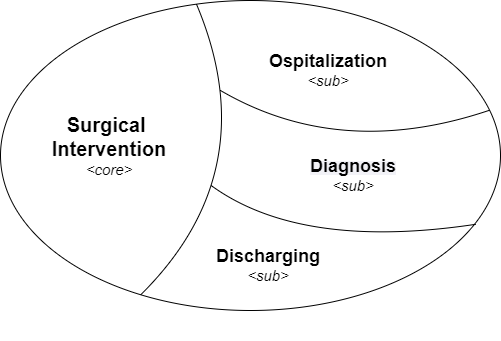
\includegraphics[width=10cm]{Images/domain_model.png}
    \centering
    \caption{\label{pic:domain-model}Dominio del nostro sistema.}
\end{figure}

\subsection{Core-Domain}
Il Core-Domain della nostra applicazione è quello che in figura \ref{pic:domain-model} abbiamo definito Surgical Intervention. Ovvero l'intervento chirurgico vero e proprio, in cui la nostra applicazione real time deve ottenere i dati dall'asset fisico (monitor dei parametri vitali presente in sala operatoria), associarlo al paziente e deve essere proiettato come ologramma interattivo sugli occhiali Hololens del personale.\newline \newline Contenendo approvvigionamento dei dati, alimentazione del digital twin e presentazione dei dati, questo dominio è risultato quello principale, ma in base all'ordine delle operazioni che vengono svolte all'interno del processo ospedaliero, abbiamo evidenziato anche altri Sub-Domains che sono in qualche modo correlati o da supporto al Core-Domain.

\subsection{Sub-Domains}
Abbiamo evidenziato altri tre Sub-Domains:
\begin{itemize}
    \item \textbf{Ospitalization}: Ricovero del paziente. In questa fase viene compilata la scheda del paziente con i dati necessari all'operazione che deve eseguire.
    
    \item \textbf{Diagnosis}: Visite e analisi relative all'operazione, svolte prima e dopo l'operazione stessa.
    
    \item \textbf{Discharging}: Dimissione del paziente. Conclusa l'operazione, la scheda del paziente e le informazioni relative all'operazione vengono archiviate.
\end{itemize}

La fase di ricovero e di dimissione del paziente sono domini che in qualche modo sono di supporto al Core-Domain evidenziato.
\newline Durante il ricovero, alla creazione della scheda del paziente sarà possibile inizializzare il nostro sistema, mentre alla dimissione si potranno chiudere l'istanza del digital twin non più necessario.

\subsection{Bounded Context}

Per ogni Sub-Domain abbiamo individuato i bounded context che racchiudessero delle funzionalità indipendenti le une dalle altre.

\begin{figure}[H]
    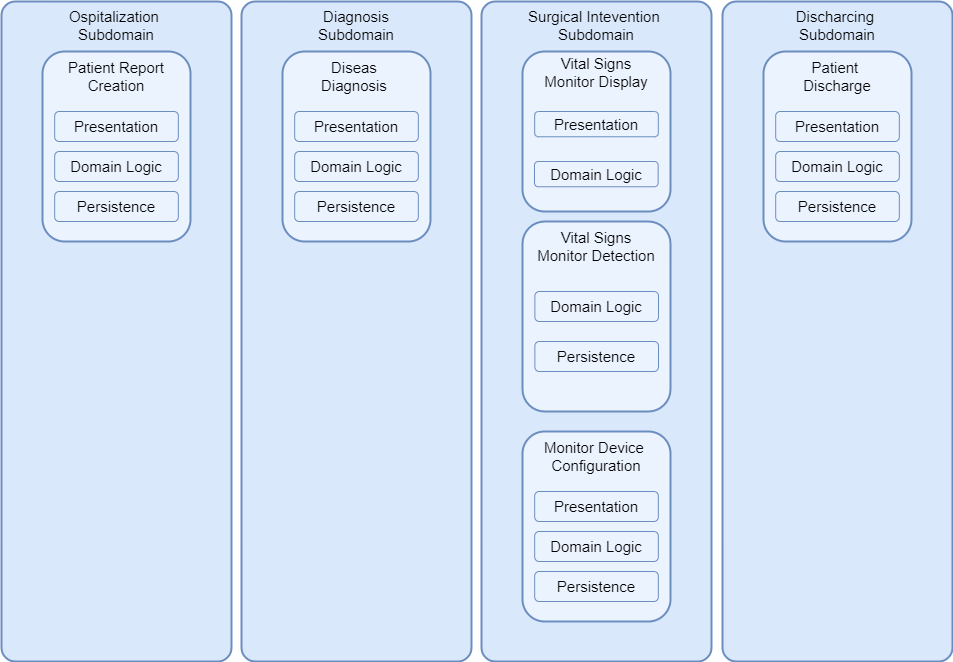
\includegraphics[width=12cm]{Images/bounded_context.png}
    \centering
    \caption{\label{pic:bounded-context}Bounded context evidenziati.}
\end{figure}

Come mostrato in figura     \ref{pic:bounded-context}, il \textit{Surgical Intevention Subdomain} è suddiviso in tre diversi Bounded Context:

\begin{itemize}
    \item \textbf{Vital Signs Monitor Display}: Visualizzazione del digital twin del monitor parametri vitali ed interazione con esso;
    \item \textbf{Vital Signs Monitor Detection}: Rilevazione dei parametri vitali del paziente e della verifica del superamento delle soglie di allarme;
    \item \textbf{Monitor Device Configuration}: Configurazione dell'asset fisico. 
\end{itemize}